% !TEX program = xelatex
% c5p-s-2026-answer.tex
% 2026 €€£ 非专业级别软件能力认证第一轮（C5P-S1）提高级 C++语言试题·参考答案与解析
% 自制模拟卷，非官方试题；编译：xelatex c5p-s-2026-answer.tex（建议编译两次）
\documentclass[a4paper]{ctexart}
\usepackage{fontspec}
\usepackage{geometry}
\usepackage{amsmath}
\usepackage{amssymb}
\usepackage{booktabs}
\usepackage{longtable}
\usepackage{array}
\usepackage{enumitem}
\usepackage{fancyhdr}
\usepackage{lastpage}
\usepackage{tikz}
\usetikzlibrary{arrows.meta,positioning}
\geometry{top=2.4cm, left=1.9cm, right=1.9cm, bottom=2.9cm}
\setmainfont{Consolas}
\setCJKmainfont[BoldFont=SimHei]{SimSun}
\newCJKfontfamily{\dengxian}{DengXian}
\DeclareMathSizes{10.53937}{10.95}{7.5}{5.5}
\setlength{\parindent}{0pt}
\setlength{\parskip}{3pt}
\linespread{1.25}
\newcommand{\ans}[2]{\noindent\textbf{#1} \quad 答案：#2\par}
\newcommand{\expn}[1]{\hspace*{1.5em}解析：#1\par}
\newcommand{\bigtitle}[1]{\begin{center}\dengxian\large #1\end{center}}
\newcommand{\overview}[1]{\par\smallskip\noindent\textbf{题目在做什么：}#1\par\smallskip}
\pagestyle{fancy}
\fancyhf{}
\fancyfoot[C]{€€£ C5P-S 2026 参考答案与解析\\第\thepage 页，共\pageref{LastPage}页}
\renewcommand{\headrulewidth}{0pt}
\renewcommand{\footrulewidth}{0pt}

\begin{document}

\begin{center}
{\dengxian
    {\xeCJKsetup{CJKecglue={\hskip 0.419em}}\fontsize{15.95}{1}\selectfont 2026 €€£非专业级别软件能力认证第一轮}\\[1em]
    {\xeCJKsetup{CJKecglue={\hskip 0.419em}}\fontsize{14.05}{1}\selectfont （C5P-S1）提高级 C++语言试题 \textbf{参考答案与解析}}
}
\end{center}

\noindent\textbf{说明：}本文件对应自制模拟卷，不代表任何官方机构。知识点级别依据《全国青少年信息学奥林匹克系列竞赛大纲（2025 年修订版）》；题目难度是本卷内部估计，不是考纲对具体题目的官方评级。

\section*{分值与题号}
\begin{center}
\begin{tabular}{c c c c}
\toprule
部分 & 题号 & 题量与计分 & 小计\\
\midrule
单项选择 & 1--15 & $15\times2$ 分 & 30 分\\
阅读程序（1） & 16--21 & $4\times1.5+2\times3$ 分 & 12 分\\
阅读程序（2） & 22--27 & $3\times1.5+3\times3$ 分 & 13.5 分\\
阅读程序（3） & 28--33 & $3\times1.5+2\times3+1\times4$ 分 & 14.5 分\\
完善程序 & 34--43 & $10\times3$ 分 & 30 分\\
\midrule
\multicolumn{3}{r}{总分} & 100 分\\
\bottomrule
\end{tabular}
\end{center}

\section*{一、单项选择题（1--15）}
\ans{1.}{B}
\expn{\texttt{cat} 是 concatenate 的缩写，用于连接并显示文件内容；\texttt{cp} 复制文件，\texttt{ping} 检查网络连通性，\texttt{touch} 创建文件或更新时间戳。知识点：Linux 文件操作；难度：5。}
\ans{2.}{C}
\expn{哈夫曼树没有度为 1 的结点。\texttt{m} 个叶子对应 \texttt{2m-1} 个结点和 \texttt{2m-2} 条边。二叉链表共有 \texttt{2(2m-1)} 个指针域，非空指针有 \texttt{2m-2} 个，因此空指针域为 \texttt{2m}。知识点：树的性质；难度：4。}
\ans{3.}{B}
\expn{完全二叉树的高度为 $O(\log n)$，叶子数量为 $O(n)$；对每个叶子向根访问一次，总访问量为 $O(n\log n)$。知识点：复杂度分析；难度：6。}
\ans{4.}{D}
\expn{把向右记为 1、向上记为 0，条件 \texttt{x >= y} 表示任意前缀中 1 不少于 0。长度为 10 的合法括号序列数量为卡特兰数 $C_5=\frac{1}{6}\binom{10}{5}=42$。知识点：组合数学；难度：7。}
\ans{5.}{A}
\expn{栈 A 中底部元素最早进入。只有在栈 B 为空时把 A 整体倒入 B，才能把最早元素放到 B 的栈顶；B 非空时直接弹出即可。知识点：栈与队列模拟；难度：3。}
\ans{6.}{C}
\expn{设选出的数为 $x_1<x_2<x_3<x_4$。因为相邻不能同时选，令 $y_i=x_i-(i-1)$，则 $1\le y_1<y_2<y_3<y_4\le7$。所以答案为 $\binom74=35$。知识点：不相邻组合计数；难度：6。}
\ans{7.}{C}
\expn{\texttt{set} 中元素按键值自动有序且不重复，基于平衡树时插入、删除和查找均为 $O(\log n)$。\texttt{map} 按键有序，键也不能重复。知识点：STL 容器；难度：5。}
\ans{8.}{C}
\expn{拓扑序要求每条边的起点排在终点之前；有环时不存在拓扑序，拓扑序也不等同于一次 DFS 序列。知识点：拓扑排序；难度：6。}
\ans{9.}{A}
\expn{\texttt{next} 数组记录模式串失配时可以回退到的最长公共前后缀位置，使主串指针不必回退。知识点：KMP；难度：6。}
\ans{10.}{A}
\expn{不使用堆时，每轮在线性时间内寻找当前最小的未确定顶点，并进行松弛，总复杂度为 $O(n^2)$。知识点：Dijkstra；难度：6。}
\ans{11.}{D}
\expn{设 $p=20260913$。模 $p$ 下，$1/k+1/(p-k)\equiv0$，所以 $1$ 到 $p-1$ 的倒数和为 0。题目缺少 $1/1$，括号内为 $-1\equiv p-1$；指数 $p$ 为奇数，结果仍为 $-1\equiv20260912$。知识点：模运算；难度：7。}
\ans{12.}{C}
\expn{单位区间上两点距离的期望是 $1/3$，线性放大到长度 2 后期望也放大 2 倍，得到 $2/3$。知识点：概率期望；难度：5。}
\ans{13.}{C}
\expn{图中共有 9 条边。所有从 1 到 8 的路径都必须经过 $4\to5$ 和 $7\to8$，删除任意一条时这两条边都会使可达性断开。其余 7 条边各有替代路径，因此可以删除的边共有 $9-2=7$ 条。\par
\begin{center}
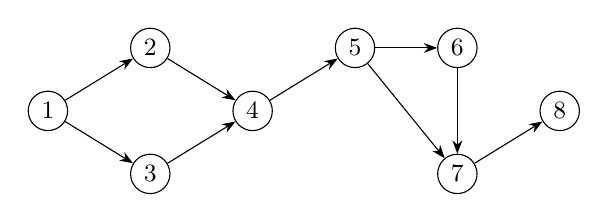
\begin{tikzpicture}[>=Stealth, every node/.style={circle, draw, fill=white, minimum size=5mm, inner sep=0.5pt, font=\small}]
\node (a) at (0,0) {1}; \node (b) at (1.3,0.8) {2}; \node (c) at (1.3,-0.8) {3}; \node (d) at (2.6,0) {4};
\node (e) at (3.9,0.8) {5}; \node (f) at (5.2,0.8) {6}; \node (g) at (5.2,-0.8) {7}; \node (h) at (6.5,0) {8};
\draw[->] (a)--(b); \draw[->] (a)--(c); \draw[->] (b)--(d); \draw[->] (c)--(d); \draw[->] (d)--(e); \draw[->] (e)--(f); \draw[->] (e)--(g); \draw[->] (f)--(g); \draw[->] (g)--(h);
\end{tikzpicture}
\end{center}
知识点：有向图可达性与必经边；难度：7。}
\ans{14.}{B}
\expn{用容斥原理：$200-(100+66+28)+(33+14+9)-4=58$。知识点：容斥原理；难度：7。}
\ans{15.}{A}
\expn{第 $i$ 层有 $k^{i-1}$ 个结点，总数为 $1+k+\cdots+k^{h-1}=\frac{k^h-1}{k-1}$。知识点：树的性质；难度：3。}

\section*{二、阅读程序（16--33）}
\subsection*{（1）归并排序}
\overview{程序先递归地把区间分成左右两半，直到区间只有一个元素；返回时把两个已经有序的子区间合并。\texttt{mid} 是分界点，\texttt{i,j} 指向两个子区间当前未处理位置，\texttt{k} 指向临时数组的写入位置。每次合并结束后，再把 \texttt{tmp[l..r]} 写回 \texttt{a[l..r]}。}
\begin{center}
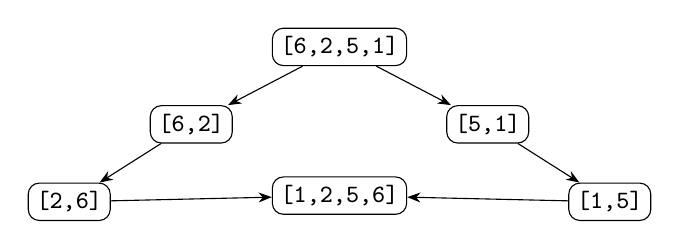
\begin{tikzpicture}[>=Stealth, node distance=7mm, every node/.style={draw, rounded corners, inner sep=3pt, font=\small}]
\node (a) {\texttt{[6,2,5,1]}};
\node (b) [below left=of a] {\texttt{[6,2]}}; \node (c) [below right=of a] {\texttt{[5,1]}};
\node (d) [below left=of b] {\texttt{[2,6]}}; \node (e) [below right=of c] {\texttt{[1,5]}};
\node (f) [below=14mm of a] {\texttt{[1,2,5,6]}};
\draw[->] (a)--(b); \draw[->] (a)--(c); \draw[->] (b)--(d); \draw[->] (c)--(e); \draw[->] (d)--(f); \draw[->] (e)--(f);
\end{tikzpicture}
\end{center}
\ans{16.}{A（√）}\expn{递归继续划分，单元素区间天然有序；合并两个有序区间后仍有序，因此最终整个数组非降序。}
\ans{17.}{A（√）}\expn{两个子区间的当前元素分别是各自剩余部分的最小值，选择较小者写入 \texttt{tmp}，正是归并的核心。相等时取左边元素还保持稳定性。}
\ans{18.}{B（×）}\expn{每次只保证当前区间的 \texttt{tmp[l..r]} 被写满；区间外的数组位置可能没有本轮意义上的结果，所以不能说整个 \texttt{tmp[1..n]} 一定有序。}
\ans{19.}{A（√）}\expn{每层把区间长度约减半，递归树高度为 $O(\log n)$。}
\ans{20.}{B}\expn{$(1+8)>>1=4$，因此左区间为 $[1,4]$，右区间为 $[5,8]$。}
\ans{21.}{B}\expn{每一层所有合并操作总共处理 $O(n)$ 个元素，共有 $O(\log n)$ 层，时间复杂度为 $O(n\log n)$；临时数组占 $O(n)$ 额外空间，递归栈为 $O(\log n)$。}

\subsection*{（2）字典序最小子序列}
\overview{程序维护一个单调栈。扫描新字符时，如果栈顶字符更大且还允许删除，就删除栈顶，让更小的当前字符尽量靠前；扫描结束仍有删除次数时，从末尾删除，因为前缀已经不能再通过前大后小的逆序得到改善。}
\begin{center}
\begin{tabular}{c c c c c c c c}
\toprule
读入 & c & b & a & c & d & c & a\\
栈变化 & c & b & a & ac & acd & acd & acda\\
\bottomrule
\end{tabular}
\end{center}
\ans{22.}{A（√）}\expn{每次删除都优先消除更靠前位置的逆序，得到的结果在字典序上更小，且总共恰好删除 \texttt{k} 个字符。}
\ans{23.}{B（×）}\expn{应在 \texttt{st.back() > ch} 时弹栈。若栈顶更小，保留更小字符在前面反而更优。}
\ans{24.}{A（√）}\expn{若扫描结束仍有删除次数，说明栈中已经没有可改善的前大后小位置；继续删除末尾不会改变已确定的更优前缀。}
\ans{25.}{A}\expn{在最坏情况下字符始终非降序，几乎不会弹栈，所有 $n$ 个字符都可能同时留在 \texttt{st} 中。}
\ans{26.}{A}\expn{处理 \texttt{cbacdca} 并删除 3 个字符时，依次弹出前面的 \texttt{c}、\texttt{b} 和后面的 \texttt{d}，栈中剩下 \texttt{acca}。}
\ans{27.}{A}\expn{每个字符最多入栈一次、出栈一次，虽然有 while 循环，但总弹栈次数不超过 $n$，因此总时间为 $O(n)$，空间为 $O(n)$。}

\subsection*{（3）树的直径}
\overview{第一次 BFS 从结点 1 出发，找到一个最远结点 \texttt{s}；在树中，这样的结点可以作为某条直径的端点。第二次从 \texttt{s} 出发，最远结点 \texttt{t} 到 \texttt{s} 的距离就是直径。\texttt{dista} 既记录 BFS 层数，也用 $-1$ 表示尚未访问。}
\begin{center}
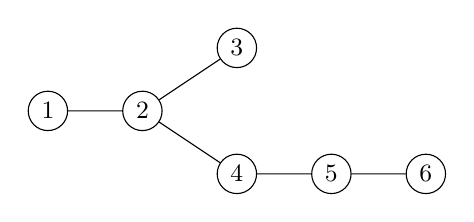
\begin{tikzpicture}[every node/.style={circle, draw, fill=white, minimum size=5mm, inner sep=0.5pt, font=\small}]
\node (a) at (0,0) {1}; \node (b) at (1.2,0) {2}; \node (c) at (2.4,0.8) {3}; \node (d) at (2.4,-0.8) {4};
\node (e) at (3.6,-0.8) {5}; \node (f) at (4.8,-0.8) {6};
\draw (a)--(b)--(c); \draw (b)--(d)--(e)--(f);
\end{tikzpicture}
\quad\text{直径端点可以是 3 和 6，长度为 4}
\end{center}
\ans{28.}{A（√）}\expn{树中从任意点出发到最远点的路径会延伸到某条直径的端点；因此第一次 BFS 得到的 \texttt{s} 可作为第二次 BFS 的起点。}
\ans{29.}{A（√）}\expn{第二次 BFS 计算了从 \texttt{s} 到所有点的距离，最大值 \texttt{dista[t]} 就是两端点之间的最长距离，即树的直径。}
\ans{30.}{A（√）}\expn{每条无向边输入一次，但调用 \texttt{add} 两次分别存储两个方向，所以邻接项数为 $2(n-1)$。}
\ans{31.}{B}\expn{当前队列尾位置为 \texttt{r}，先把 \texttt{v} 写到 \texttt{que[r]}，再令 \texttt{r} 加一，合写为 \texttt{que[r++] = v;}。}
\ans{32.}{C}\expn{BFS 中 $-1$ 同时表示“未访问”。访问邻居时判断 \texttt{dista[v] == -1}，可避免重复入队。}
\ans{33.}{B（4 分）}\expn{第二次 BFS 计算的树上最长路径为 $1\to2\to4\to5\to6$，包含 4 条边，因此输出 4。}

\section*{三、完善程序（34--43）}
\subsection*{（1）有序序列的第 K 小和}
\overview{对固定的和 \texttt{sum}，\texttt{count\_le(sum)} 统计不超过它的数对数量。由于这个数量随 \texttt{sum} 增大而不减，可以在答案范围上二分第一个使数量不少于 \texttt{k} 的值。内层用 upper bound 统计每个 \texttt{a[i]} 能匹配多少个 \texttt{b[j]}。}
\begin{center}
\begin{tikzpicture}[>=Stealth, every node/.style={draw, rounded corners, inner sep=4pt, font=\small}]
\node (x) {候选和 \texttt{mid}}; \node (y) [right=18mm of x] {统计 \texttt{count\_le(mid)}}; \node (z) [right=18mm of y] {与 \texttt{k} 比较};
\draw[->] (x)--(y); \draw[->] (y)--(z); \draw[->] (z) to[bend left=18] node[above]{不少于} (x); \draw[->] (z) to[bend right=18] node[below]{少于} (x);
\end{tikzpicture}
\end{center}
\ans{34.}{A}\expn{半开区间 $[0,n)$ 的右端点应初始化为 \texttt{n}。}
\ans{35.}{A}\expn{upper bound 要找第一个严格大于 \texttt{x} 的位置，所以判断条件是 \texttt{a[mid] > x}。}
\ans{36.}{A}\expn{循环结束时 \texttt{l == r}，这个位置就是第一个大于 \texttt{x} 的下标，也就是不超过 \texttt{x} 的元素个数。}
\ans{37.}{A}\expn{所有数对和的最小值由两个序列的首元素相加得到，即 \texttt{a[0]+b[0]}。}
\ans{38.}{A}\expn{最大值由两个序列的末元素相加得到，即 \texttt{a[n-1]+b[n-1]}；二分在闭区间答案范围内进行。}

\subsection*{（2）最小生成树}
\overview{Kruskal 按边权从小到大扫描边。并查集维护当前每个结点所属的连通分量：若一条边的两个端点已经在同一集合中，加入它会形成环，应跳过；否则合并两个集合并把边加入生成树。最终若选中 $n-1$ 条边，则得到最小生成树。}
\begin{center}
\begin{tikzpicture}[>=Stealth, every node/.style={draw, rounded corners, inner sep=4pt, font=\small}]
\node (a) {按边权排序}; \node (b) [right=17mm of a] {检查两个根}; \node (c) [right=17mm of b] {不同集合则合并}; \node (d) [below=10mm of b] {同集合则跳过};
\draw[->] (a)--(b); \draw[->] (b)--(c); \draw[->] (b)--(d);
\end{tikzpicture}
\end{center}
\ans{39.}{A}\expn{每个结点初始时单独属于一个集合，故 \texttt{fa[i] = i}。}
\ans{40.}{A}\expn{输入的有效边下标为 $0$ 到 $m-1$，排序范围应为 \texttt{e} 到 \texttt{e+m}。}
\ans{41.}{A}\expn{若两个端点的根相同，说明它们已经连通，再加入该边会产生环，因此判断 \texttt{x == y} 后跳过。}
\ans{42.}{B}\expn{把根为 \texttt{x} 的集合挂到根为 \texttt{y} 的集合下，应写为 \texttt{fa[x] = y}。}
\ans{43.}{B}\expn{$n$ 个结点的生成树恰有 $n-1$ 条边；若 \texttt{used != n-1}，说明图不连通。}

\clearpage
\section*{附录：考点与难度核对}
\begin{center}
\begin{longtable}{c p{4.2cm} p{3.2cm} c p{5.0cm}}
\toprule
题号 & 考点 & 大纲类别 & 难度 & 说明\\
\midrule
1--5 & Linux、树、复杂度、栈队列 & 基础/数据结构 & 3--6 & 基础概念与性质\\
6 & 不相邻组合计数 & 数学与其他 & 6 & 位置变换后组合\\
7--12 & STL、拓扑、KMP、Dijkstra、模运算、期望 & 程序/算法/图论/数学 & 5--7 & 常见经典知识\\
13--15 & 有向图可达性、容斥、满 k 叉树 & 图论/数学/数据结构 & 3--7 & 图示推理与基础性质\\
16--21 & 归并排序 & 算法 & 5--6 & 分治、合并、不变量、复杂度\\
22--27 & 单调栈 & 算法/数据结构 & 5--6 & 贪心过程与均摊复杂度\\
28--33 & 树的直径与 BFS & 图论算法 & 6--8 & 两次 BFS 与路径追踪\\
34--38 & 第 K 小和 & 二分与排序 & 6--8 & 单调判定与 upper bound\\
39--43 & Kruskal 与并查集 & 图论/数据结构 & 6--8 & 环判断、合并与连通性\\
\bottomrule
\end{longtable}
\end{center}
\noindent\textbf{总分核对：}选择题 30 分，阅读程序 $12+13.5+14.5=40$ 分，完善程序 30 分，合计 100 分。

\end{document}
